\chapter{Background}\label{sec:chapter2}

In this chapter the mathematical background that later chapters rely on is introduced.

\section{Signals on the Sphere}

\begin{figure}[htpb]
	\capstart{}
	\subfloat[\(\Re\big\{\pixel{Y_{00}}\big\}\)]  % chktex 21
	{\includegraphics[trim={23 7 3 6},clip,width=.2\textwidth]{spherical_harmonic_0l_0m_L128_real.pdf}}
	\newline
	\subfloat[\(\Re\big\{\pixel{Y_{10}}\big\}\)]  % chktex 21
	{\includegraphics[trim={23 7 3 6},clip,width=.2\textwidth]{spherical_harmonic_1l_0m_L128_real.pdf}}
	%
	\subfloat[\(\Re\big\{\pixel{Y_{11}}\big\}\)]  % chktex 21
	{\includegraphics[trim={23 7 3 6},clip,width=.2\textwidth]{spherical_harmonic_1l_1m_L128_real.pdf}}
	\newline
	\subfloat[\(\Re\big\{\pixel{Y_{20}}\big\}\)]  % chktex 21
	{\includegraphics[trim={23 7 3 6},clip,width=.2\textwidth]{spherical_harmonic_2l_0m_L128_real.pdf}}
	%
	\subfloat[\(\Re\big\{\pixel{Y_{21}}\big\}\)]  % chktex 21
	{\includegraphics[trim={23 7 3 6},clip,width=.2\textwidth]{spherical_harmonic_2l_1m_L128_real.pdf}}
	%
	\subfloat[\(\Re\big\{\pixel{Y_{22}}\big\}\)]  % chktex 21
	{\includegraphics[trim={23 7 3 6},clip,width=.2\textwidth]{spherical_harmonic_2l_2m_L128_real.pdf}}
	\newline
	\subfloat[\(\Re\big\{\pixel{Y_{30}}\big\}\)]  % chktex 21
	{\includegraphics[trim={23 7 3 6},clip,width=.2\textwidth]{spherical_harmonic_3l_0m_L128_real.pdf}}
	%
	\subfloat[\(\Re\big\{\pixel{Y_{31}}\big\}\)]  % chktex 21
	{\includegraphics[trim={23 7 3 6},clip,width=.2\textwidth]{spherical_harmonic_3l_1m_L128_real.pdf}}
	%
	\subfloat[\(\Re\big\{\pixel{Y_{32}}\big\}\)]  % chktex 21
	{\includegraphics[trim={23 7 3 6},clip,width=.2\textwidth]{spherical_harmonic_3l_2m_L128_real.pdf}}
	%
	\subfloat[\(\Re\big\{\pixel{Y_{33}}\big\}\)]  % chktex 21
	{\includegraphics[trim={23 7 3 6},clip,width=.2\textwidth]{spherical_harmonic_3l_3m_L128_real.pdf}}
	\newline
	\subfloat[\(\Re\big\{\pixel{Y_{40}}\big\}\)]  % chktex 21
	{\includegraphics[trim={23 7 3 6},clip,width=.2\textwidth]{spherical_harmonic_4l_0m_L128_real.pdf}}
	%
	\subfloat[\(\Re\big\{\pixel{Y_{41}}\big\}\)]  % chktex 21
	{\includegraphics[trim={23 7 3 6},clip,width=.2\textwidth]{spherical_harmonic_4l_1m_L128_real.pdf}}
	%
	\subfloat[\(\Re\big\{\pixel{Y_{42}}\big\}\)]  % chktex 21
	{\includegraphics[trim={23 7 3 6},clip,width=.2\textwidth]{spherical_harmonic_4l_2m_L128_real.pdf}}
	%
	\subfloat[\(\Re\big\{\pixel{Y_{43}}\big\}\)]  % chktex 21
	{\includegraphics[trim={23 7 3 6},clip,width=.2\textwidth]{spherical_harmonic_4l_3m_L128_real.pdf}}
	%
	\subfloat[\(\Re\big\{\pixel{Y_{44}}\big\}\)]  % chktex 21
	{\includegraphics[trim={23 7 3 6},clip,width=.2\textwidth]{spherical_harmonic_4l_4m_L128_real.pdf}}
	\caption[
		The spherical harmonics for \(\ell=0,1,2,3,4\)
	]{
		The real part of the spherical harmonics \(\pixel{\harmonic{Y}}\) for \(\ell=0,1,2,3,4\) (top-to-bottom) and \(m=0,\ldots,\ell{}\) (left-to-right).
		The negative order harmonics \(\pixel{Y_{\ell(-m)}}\) have not been included as they are simply rotated with respect to the positive order harmonics by \(\SI{90}{\degree}/m\).
	}\label{fig:chapter2_spherical_harmonics}
\end{figure}


\section{Wavelets}

\subsection{Euclidean}

\subsection{Sphere}

\begin{figure}[htpb]
	\centering\capstart{}
	\subfloat[\(\pixel{\Phi}\)]
	{\includegraphics[trim={23 7 3 6},clip,width=.33\textwidth]{axisymmetric_wavelets_3B_2jmin_scaling_L128_res512_real.pdf}}
	\hfill
	\subfloat[\(\pixel{\Psi^{2j}}\)]
	{\includegraphics[trim={23 7 3 6},clip,width=.33\textwidth]{axisymmetric_wavelets_3B_2jmin_2j_L128_res512_real.pdf}}
	\hfill
	\subfloat[\(\pixel{\Psi^{3j}}\)]
	{\includegraphics[trim={23 7 3 6},clip,width=.33\textwidth]{axisymmetric_wavelets_3B_2jmin_3j_L128_res512_real.pdf}}
	\newline
	\subfloat[\(\pixel{\Psi^{4j}}\)]
	{\includegraphics[trim={23 7 3 6},clip,width=.33\textwidth]{axisymmetric_wavelets_3B_2jmin_4j_L128_res512_real.pdf}}
	%
	\subfloat[\(\pixel{\Psi^{5j}}\)]
	{\includegraphics[trim={23 7 3 6},clip,width=.33\textwidth]{axisymmetric_wavelets_3B_2jmin_5j_L128_res512_real.pdf}}
	\caption[
		Some axisymmetric scale-discretised wavelets on the sphere
	]{
		The scaling function and the wavelets for scales \(j \in \set{2, 3, 4, 5}\) of the axisymmetric scale-discretised wavelets on the sphere shown left-to-right, top-to-bottom.
		They are constructed through a tiling of the harmonic line with parameters \(\lambda=3\), \(J_{0}=2\), and bandlimit \(L=128\) (\cf{} \cref{fig:chapter2_tiling}).
	}\label{fig:chapter2_wavelets}
\end{figure}


\section{Spectral Concentration Problem}

\subsection{Euclidean}

Before considering the Slepian spatial-spectral concentration problem in the spherical domain, first consider the one-dimensional, continuous-continuous, time-frequency concentration problem.
Here, a normalisation convention is adopted such that a real-valued time-domain single \(f(t)\) and its Fourier transform \(F(\omega)\) are related by
%
\begin{equation}
	f(t)
	%
	= \frac{1}{2\pi} \int\limits_{\infty}^{\infty} F(\omega) \exp(i\omega t) \dd{\omega}
\end{equation}
%
and
%
\begin{equation}
	F(\omega)
	%
	= \int\limits_{\infty}^{\infty} f(t) \exp(-i\omega t) \dd{\omega},
\end{equation}
%
where \(t\) and \(\omega{}\) denote the time and angular frequency respectively.
Slepian and Pollak~\cite{Slepian1961} considered the problem of optimally concentrating a strictly bandlimited signal \(f(t)\), with a spectrum \(F(\omega)\) which disappears into a time interval \(\abs{t} < T\) for frequencies \(\abs{\omega} < W\).
As a result of the \emph{Paley-Wiener} theorem, no bandlimited signal \(f(t)\) can be perfectly concentrated within a finite interval~\cite{Daubechies1992,Mallat2008}.
A signal is considered optimally concentrated if it has the least energy outside the interval
%
\begin{equation}
	\mu
	%
	= \frac{\int\limits_{-T}^{T} f^{2}(t) \dd{t}}{\int\limits_{-\infty}^{\infty} f^{2}(t) \dd{t}}
\end{equation}

~\cite{Freeden1997,Riedel1995}.

\subsection{Sphere}

\begin{figure}[htpb]
	\centering\capstart{}
	\subfloat[\(\mu_{1}=1.000000\) \newline
        \(m=0\)]
	{\includegraphics[trim={23 7 3 6},clip,width=.25\textwidth]{slepian_polar40_m0_rank0_lam1-000000e00_L16_res128_real_norm.pdf}} % chktex 8
    \hfill
	\subfloat[\(\mu_{1}=0.999998\) \newline
        \(m=1\)]
	{\includegraphics[trim={23 7 3 6},clip,width=.25\textwidth]{slepian_polar40_m1_rank2_lam9-999984e-01_L16_res128_real_norm.pdf}} % chktex 8
	\hfill
	\subfloat[\(\mu_{1}=0.999998\) \newline
        \(m=-1\)]
	{\includegraphics[trim={23 7 3 6},clip,width=.25\textwidth]{slepian_polar40_m-1_rank1_lam9-999984e-01_L16_res128_real_norm.pdf}} % chktex 8
    \hfill
    \subfloat[\(\mu_{1}=0.999966\) \newline
    \(m=2\)]
    {\includegraphics[trim={23 7 3 6},clip,width=.25\textwidth]{slepian_polar40_m2_rank4_lam9-999664e-01_L16_res128_real_norm.pdf}} % chktex 8
    \newline
    \subfloat[\(\mu_{1}=0.999966\) \newline
    \(m=-2\)]
    {\includegraphics[trim={23 7 3 6},clip,width=.25\textwidth]{slepian_polar40_m-2_rank3_lam9-999664e-01_L16_res128_real_norm.pdf}} % chktex 8
    \hfill
	\subfloat[\(\mu_{2}=0.999939\) \newline
        \(m=0\)]
	{\includegraphics[trim={23 7 3 6},clip,width=.25\textwidth]{slepian_polar40_m0_rank5_lam9-999392e-01_L16_res128_real_norm.pdf}} % chktex 8
    \hfill
    \subfloat[\(\mu_{1}=0.999553\) \newline
    \(m=3\)]
    {\includegraphics[trim={23 7 3 6},clip,width=.25\textwidth]{slepian_polar40_m3_rank7_lam9-995528e-01_L16_res128_real_norm.pdf}} % chktex 8
    \hfill
	\subfloat[\(\mu_{1}=0.999553\) \newline
        \(m=-3\)]
	{\includegraphics[trim={23 7 3 6},clip,width=.25\textwidth]{slepian_polar40_m-3_rank6_lam9-995528e-01_L16_res128_real_norm.pdf}} % chktex 8
    \newline
    \subfloat[\(\mu_{2}=0.998918\) \newline
    \(m=1\)]
    {\includegraphics[trim={23 7 3 6},clip,width=.25\textwidth]{slepian_polar40_m1_rank9_lam9-989180e-01_L16_res128_real_norm.pdf}} % chktex 8
    \hfill
	\subfloat[\(\mu_{2}=0.998918\) \newline
        \(m=-1\)]
	{\includegraphics[trim={23 7 3 6},clip,width=.25\textwidth]{slepian_polar40_m-1_rank8_lam9-989180e-01_L16_res128_real_norm.pdf}} % chktex 8
    \hfill
    \subfloat[\(\mu_{1}=0.995897\) \newline
    \(m=4\)]
    {\includegraphics[trim={23 7 3 6},clip,width=.25\textwidth]{slepian_polar40_m4_rank11_lam9-958971e-01_L16_res128_real_norm.pdf}} % chktex 8
    \hfill
	\subfloat[\(\mu_{1}=0.995897\) \newline
        \(m=-4\)]
	{\includegraphics[trim={23 7 3 6},clip,width=.25\textwidth]{slepian_polar40_m-4_rank10_lam9-958971e-01_L16_res128_real_norm.pdf}} % chktex 8
    \newline
    \subfloat[\(\mu_{2}=0.988469\) \newline
    \(m=2\)]
    {\includegraphics[trim={23 7 3 6},clip,width=.25\textwidth]{slepian_polar40_m2_rank12_lam9-884688e-01_L16_res128_real_norm.pdf}} % chktex 8
    \hfill
    \subfloat[\(\mu_{2}=0.988469\) \newline
    \(m=-2\)]
    {\includegraphics[trim={23 7 3 6},clip,width=.25\textwidth]{slepian_polar40_m-2_rank13_lam9-884688e-01_L16_res128_real_norm.pdf}} % chktex 8
    \hfill
	\subfloat[\(\mu_{3}=0.984654\) \newline
        \(m=0\)]
	{\includegraphics[trim={23 7 3 6},clip,width=.25\textwidth]{slepian_polar40_m0_rank14_lam9-846542e-01_L16_res128_real_norm.pdf}} % chktex 8
    \hfill
	\subfloat[\(\mu_{1}=0.973439\) \newline
        \(m=5\)]
	{\includegraphics[trim={23 7 3 6},clip,width=.25\textwidth]{slepian_polar40_m5_rank15_lam9-734390e-01_L16_res128_real_norm.pdf}} % chktex 8
	\caption[
		The Slepian functions within a \(\SI{40}{\degree}\) polar cap
	]{
        The real part of the first sixteen Slepian functions \(\pixel{\slepian{S}}\) within a polar cap of colatitudinal radius \(\SI{40}{\degree}\).
        The bandlimit here is  \(L=16\), which corresponds to a Shannon number of \(N=30\).
        Subscripts on the eigenvalues \(\mu_{\alpha}\) denote the rank of the order \(m\), \ie{} \(\mu_{1}\) appears before \(\mu_{2}\) for a given \(m\).
        The plots are ordered by decreasing eigenvalue shown left-to-right, top-to-bottom --- indicating worse concentration within the region.
        Note the similarity with the spherical harmonics in this straightforward region.
	}\label{fig:chapter2_slepian_polar_cap}
\end{figure}


\begin{figure}[htpb]
	\centering\capstart{}
	\includegraphics[width=\textwidth]{slepian_colatitude.pdf}
	\caption[
		The colatitudinal dependence of the polar cap Slepian functions
	]{
		The colatitudinal dependence of the Slepian functions \(\pixel{\slepian{S}}\) within a polar cap of colatitudinal radius \(\Theta=\SI{40}{\degree}\) for \(p \in \set{1, 6, 15, 30, 51, 72}\) shown left-to-right, top-to-bottom.
		The bandlimit here is  \(L=16\), which corresponds to a Shannon number of \(N=30\), \ie{} the final two panels are beyond the Shannon number.
		Blue curves show the concentration within the cap \(\SI{0}{\degree} \leq \theta \leq \Theta{}\), whilst orange curves show the leakage into the rest of the sphere \(\Theta < \theta \leq \SI{180}{\degree}\).
		The eigenvalue \(\mu{}\) quantifies the relative spatial concentration of the Slepian function, where lower values have increasing leakage into the orange curve.
	}\label{fig:chapter2_slepian_colatitude}
\end{figure}


\begin{figure}[htpb]
	\centering\capstart{}
	\includegraphics[width=\textwidth]{polar_cap_eigenvalues.pdf}
	\caption[
		The Slepian eigenvalues within a \(\SI{40}{\degree}\) polar cap
	]{
		The ordered Slepian eigenvalues within a polar cap of colatitudinal radius \(\SI{40}{\degree}\).
		The bandlimit here is  \(L=16\), which corresponds to a Shannon number of \(N=30\), as indicated on the plot.
		Initially the eigenvalues are \(\almost{1}\), before decreasing rapidly around the Shannon number, and where the majority of the later eigenvalues are \(\almost{0}\).
		The different symbols represent the orders \(-15 \leq m \leq 15\), where adjacent matching symbols are \(\pm m\) doublets.
	}\label{fig:chapter2_polar_cap_eigenvalues}
\end{figure}


\section{Motivation}

\subsection{Overview}

\subsection{Cosmology}

\begin{figure}[htpb]
	\centering\capstart{}
	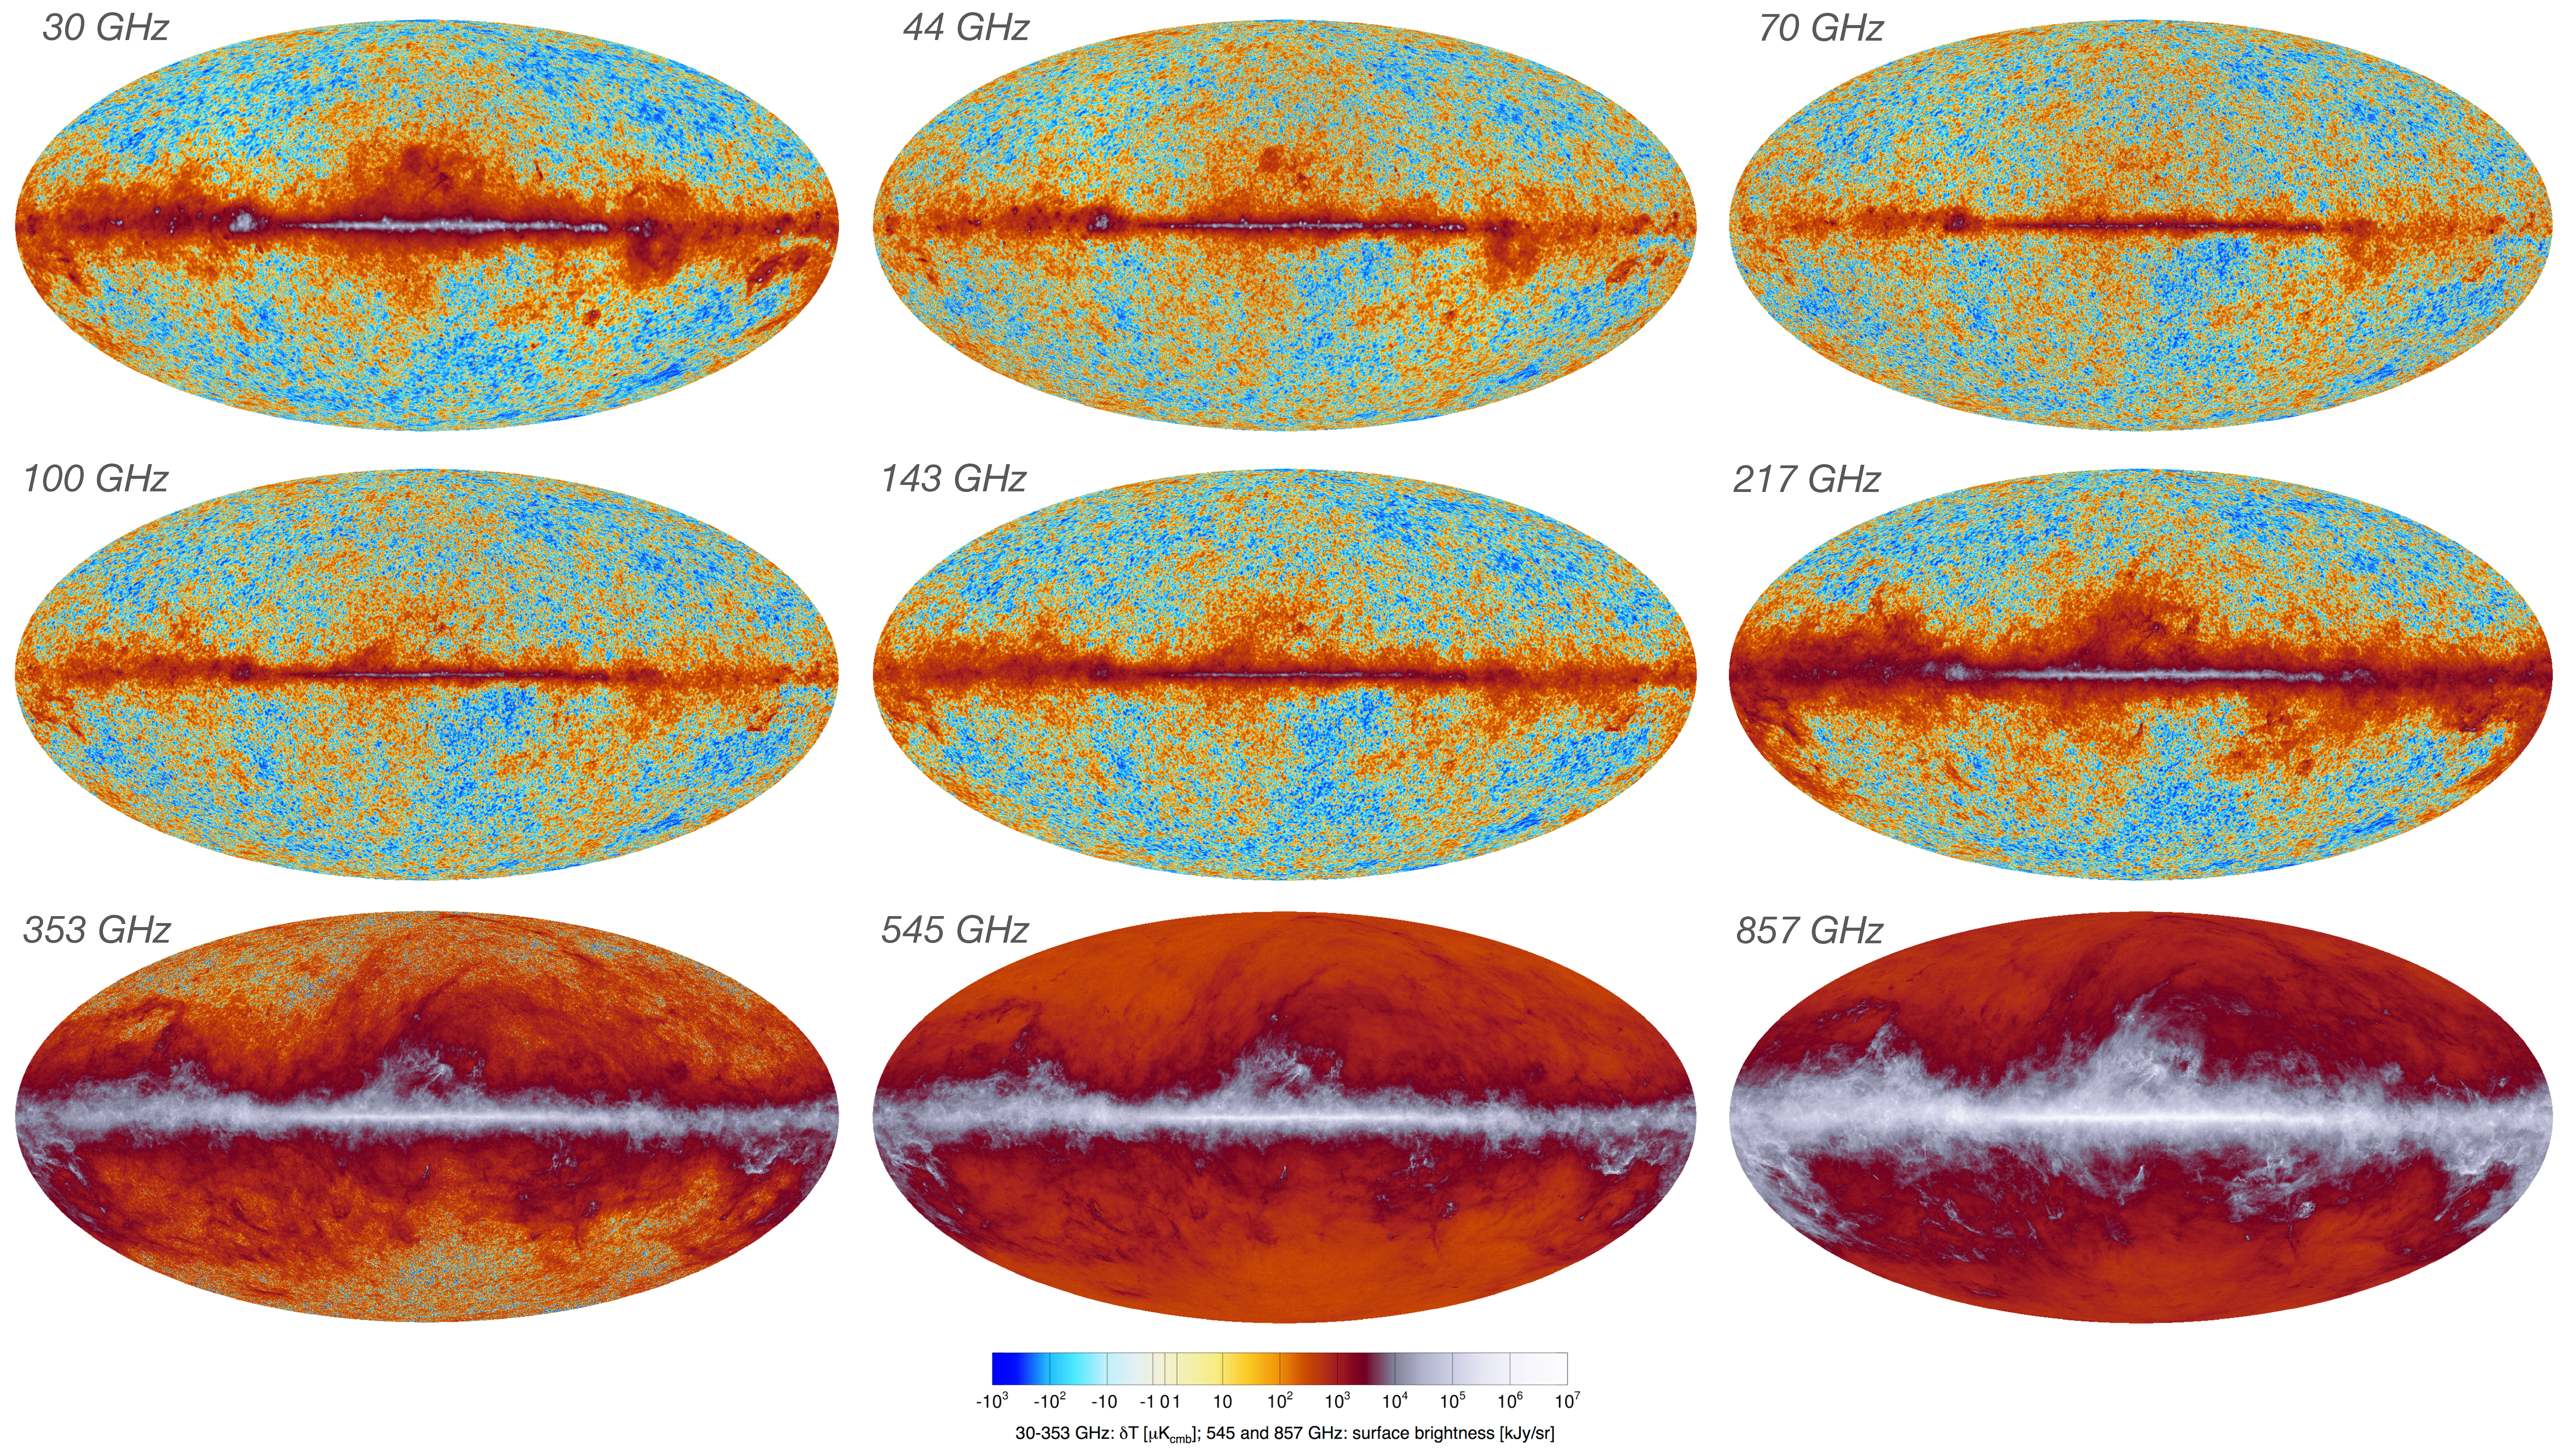
\includegraphics[width=\textwidth]{planck_2018_temp_freq.pdf}
	\caption[

	]{

	}\label{fig:chapter2_planck_frequency}
\end{figure}


\begin{figure}[htpb]
	\centering\capstart{}
	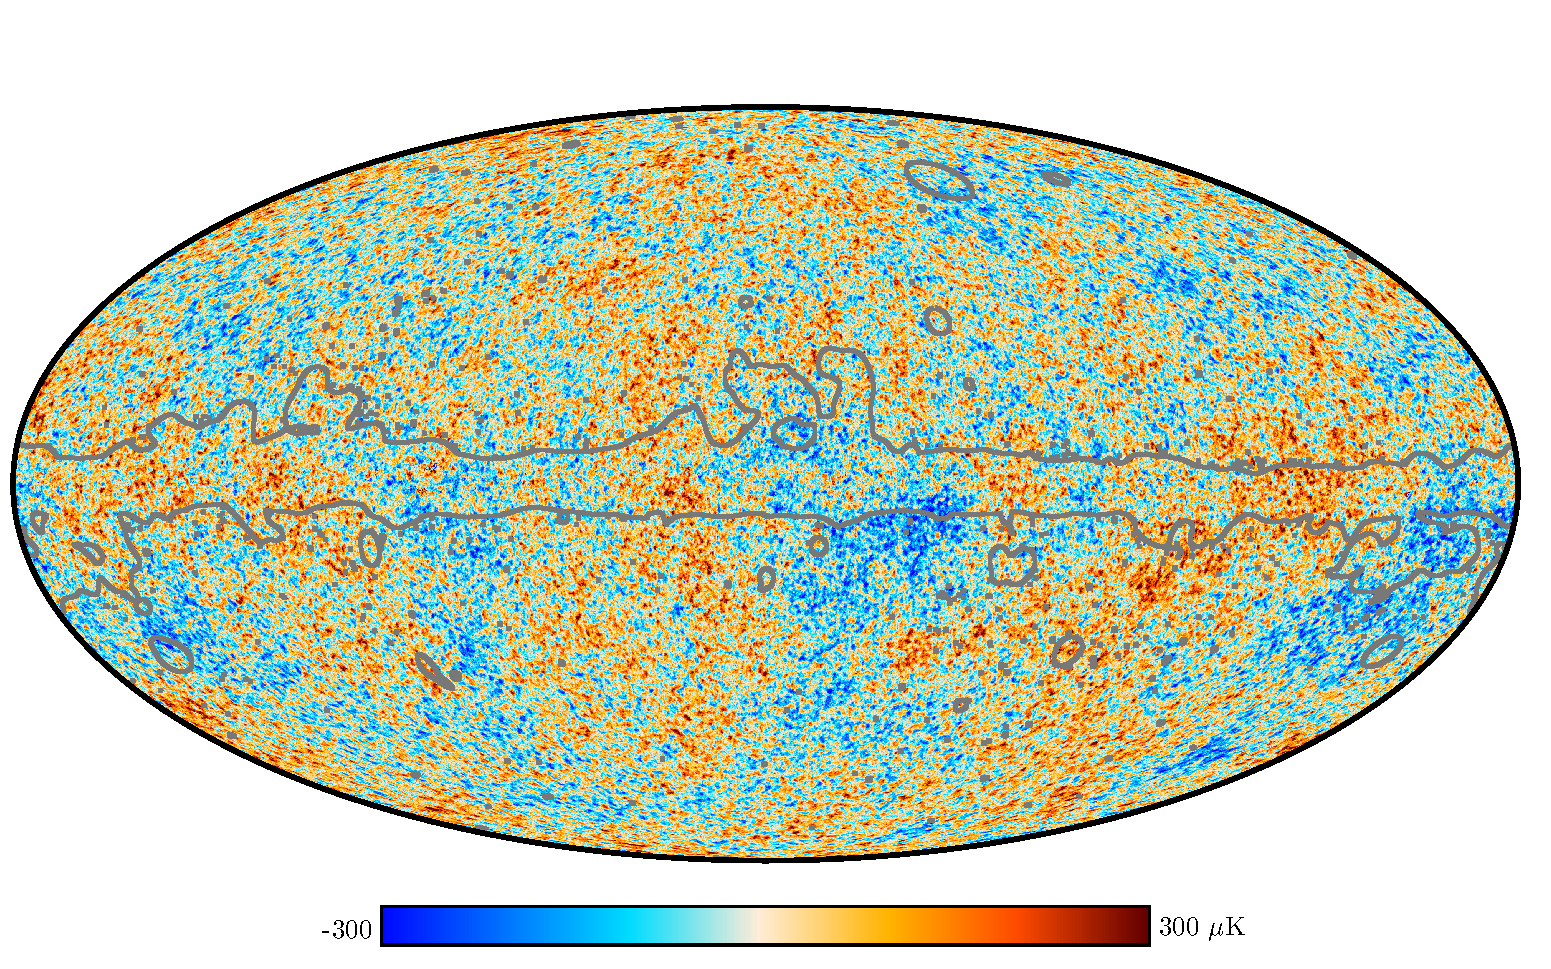
\includegraphics[width=\textwidth]{planck_2018_temp_mask.pdf}
	\caption[
		The 2018 \emph{Planck} CMB map extracted using the \texttt{SMICA} method
	]{
		The \texttt{SMICA}~\cite{Planck2020a} foreground-cleaned temperature map of the \emph{Planck} CMB sky (courtesy of \emph{The Planck Collaboration 2018}~\cite{Planck2020}).
		The CMB map has been masked, primarily around the Galactic plane (outlined in grey), and inpainted in regions where residuals from foreground emission are expected to be considerable.
		Slepian wavelets offer an alternative approach in which the wavelets are constructed in the region outside the mask.
	}\label{fig:chapter2_planck_unmasked}
\end{figure}


\subsection{Statistics of Random Fields on the Sphere}

\subsection{Observations Over the Partial Sphere}

\section{Outlook}

\subsection{Current Approaches}

\subsection{This Thesis}
